\documentclass[11pt]{article}
\usepackage[margin=1in]{geometry}
\usepackage{amsmath,amssymb}
\usepackage{graphicx}
\usepackage{booktabs}
\usepackage{hyperref}
\usepackage{xcolor}

\title{Temporal Dynamics of Viability-Constrained Memory Systems:\\
       Consolidation Burst and MID\_DECAY-Limited Forgetting}
\author{Gabriel Aubin-Moreau}
\date{2026}

\begin{document}
\maketitle

\begin{abstract}
We characterize the two temporal phases of the VCML saturation law
$\mathrm{sg4}_\infty = C \cdot \mathrm{FA} / (\mathrm{FA} + K_{\mathrm{eff}})$
(Papers 15--17): the buildup from zero to steady state during sustained wave input
(Phase~1), and the decay after wave cessation (Phase~3).
Three findings contradict naive predictions.
(i)~The \emph{buildup timescale} is long ($\sim$1600--2000 steps) and reflects
the joint bottleneck of baseline tracking ($\tau_{\mathrm{base}} = 1/\beta_{\mathrm{base}} = 200$),
mid-memory accumulation ($\tau_m = 1/(1-\delta) = 100$), and spatial diffusion.
(ii)~When wave input ceases, sg4 first \emph{rises} by $\sim$40\% before decaying:
sites that were perpetually wave-blocked and unable to consolidate
now flush their accumulated mid-memory signal, temporarily boosting inter-zone contrast.
We term this the \emph{consolidation burst}.
(iii)~The \emph{forgetting timescale} is $\tau_{\mathrm{forget}} \approx 100$--200 steps
and is governed by $\tau_m = 1/(1-\delta)$ rather than $1/\mathrm{FA}$
as one might naively expect.
Forgetting is thus MID\_DECAY-controlled, nearly FA-independent,
and counterintuitively increases with diffusion coefficient $\kappa$.
Together, these results complete the temporal portrait of the saturation law.
\end{abstract}

%----------------------------------------------------------------------
\section{Introduction}
%----------------------------------------------------------------------

Papers 15 and 16 established that the steady-state inter-zone contrast obeys
\begin{equation}
  \mathrm{sg4}_\infty = C \cdot \frac{\mathrm{FA}}{\mathrm{FA} + K_{\mathrm{eff}}},
  \quad K_{\mathrm{eff}} = \frac{\kappa}{P_{\mathrm{consol}}},
  \label{eq:sat}
\end{equation}
and Paper~17 showed that every free parameter maps onto $C$ or $K_{\mathrm{eff}}$.
Equation~\eqref{eq:sat} is a \emph{steady-state} law; it says nothing about
\emph{when} the system reaches that steady state, or how fast it forgets
when input ceases.

Two naive predictions suggest themselves:
\begin{enumerate}
\item \textbf{Buildup}: The consolidation rate per site per step is $\mathrm{FA} \cdot P_{\mathrm{consol}}$,
  so $\tau_{\mathrm{build}} \sim 1/(\mathrm{FA} \cdot P_{\mathrm{consol}})$.
  This would make buildup strongly FA-dependent.
\item \textbf{Forgetting}: In Phase~3 (no waves), all sites become calm
  and eligible ($\mathrm{streak} \geq SS$), so $F \to m$ at rate $\mathrm{FA}$ per step,
  giving $\tau_{\mathrm{forget}} \sim 1/\mathrm{FA}$.
  Both buildup and forgetting would scale the same way.
\end{enumerate}
We test these predictions directly.

%----------------------------------------------------------------------
\section{Methods}
%----------------------------------------------------------------------

\paragraph{Setup.}
We use the standard small-grid VCML substrate from Papers 15--17:
$W=40$, $H=20$, $\mathrm{HALF}=20$, $N_{\mathrm{act}}=400$,
$\mathrm{HS}=2$, four zones of width $\mathrm{ZONE\_W}=5$,
$\mathrm{BASE\_BETA}=0.005$, $\mathrm{ALPHA\_MID}=0.15$,
$\mathrm{MID\_DECAY}=0.99$, $SS=10$, $\mathrm{FD}=0.9997$,
$\nu=0.001$, $\mathrm{SEED\_BETA}=0.25$,
$\mathrm{WR}=4.8$, $\mathrm{WAVE\_DUR}=15$.

\paragraph{Protocol.}
Each run proceeds in two phases:
\begin{itemize}
  \item \textbf{Phase 1} ($t = 1$--$2000$):
    Waves launched stochastically at rate $\mathrm{WR}/\mathrm{WAVE\_DUR}$ per step.
    Top/bottom rows alternate $\pm\mathbf{d}_B$ perturbations
    ($\mathbf{d}_B = [0,\,1]$), creating a vertically structured signal
    that the copy-forward loop converts into spatial inter-zone contrast.
    sg4 is recorded every 200 steps.
  \item \textbf{Phase 3} ($t = 2001$--$2200$):
    No new waves launched. Existing waves expire.
    All sites progressively calm; the consolidation gate opens for every site.
    sg4 is recorded every 10 steps.
\end{itemize}

\paragraph{Sweep.}
$\mathrm{FA} \in \{0.10, 0.20, 0.40, 0.70\}$,
$\kappa \in \{0.005, 0.020, 0.080\}$,
5 seeds each.
Total: 60 independent runs.

\paragraph{Analysis.}
The forgetting timescale $\tau_{\mathrm{forget}}$ is estimated as the time
(from $T_{\mathrm{build}} = 2000$) for sg4 to fall to $1/e$ of its value
at $T_{\mathrm{build}}$, using linear interpolation between checkpoints.

%----------------------------------------------------------------------
\section{Results}
%----------------------------------------------------------------------

\subsection{Buildup is slow and FA-dependent in amplitude, not timescale}

Figure~1A shows sg4 vs.\ time during Phase~1 for all four FA values at $\kappa=0.020$.
Several features are apparent.

\textbf{Slow buildup.}
The system does not approach steady state until $t \approx 1600$--$2000$ steps---far longer
than the naive prediction $1/(\mathrm{FA} \cdot P_{\mathrm{consol}}) \approx 6$--$57$ steps.
The dominant bottleneck is the baseline-tracking timescale
$\tau_{\mathrm{base}} = 1/\mathrm{BASE\_BETA} = 200$ steps:
until the baseline has correctly tracked the wave-perturbed hidden state,
the contrastive signal $(h - \mathrm{base})$ is small and mid-memory accumulates slowly.

\textbf{FA-dependent amplitude.}
Higher FA produces higher steady-state sg4, consistent with Eq.~\eqref{eq:sat}.
At $t=2000$: $\mathrm{sg4} \approx 137$ (FA=0.10) vs.\ $\approx 192$ (FA=0.70).

\textbf{FA-independent timescale.}
The shape of the buildup curves is similar across FA values.
The FA ratio (0.70/0.10) produces only a $\sim$40\% difference in sg4 at $t=200$
(2.95 vs.\ 0.94), far less than the 7× ratio in FA.
The buildup timescale is governed by
$\max(\tau_{\mathrm{base}},\,\tau_m) = \max(200, 100) = 200$ steps,
not by FA.

\subsection{Consolidation burst: sg4 rises when waves stop}

Figure~1B shows sg4 normalized to its value at $T_{\mathrm{build}}=2000$,
as a function of time after wave cessation.
The most striking feature is that sg4 \emph{increases} by approximately 40\%
in the first 30 steps of Phase~3, before beginning to decay.

We term this the \textbf{consolidation burst}.
During Phase~1, a significant fraction of sites are wave-perturbed repeatedly
and never accumulate a calm streak long enough to reach the consolidation gate
($\mathrm{streak} \geq SS = 10$).
These sites hold accumulated mid-memory signal but cannot write it to fieldM.
When waves cease, all sites become calm.
Within $\sim$SS steps, the blocked sites gain eligibility and flush their mid-memory
into fieldM, transiently boosting inter-zone contrast above the Phase~1 level.

The consolidation burst is visible for all FA values and has approximately equal magnitude,
confirming that it is a gate-opening effect driven by geometry ($SS$, wave density),
not by FA.

\subsection{Forgetting is MID\_DECAY-limited, not FA-limited}

After the consolidation burst, sg4 decays approximately exponentially.
The forgetting timescale (Table~\ref{tab:tau}) is $\tau_{\mathrm{forget}} \approx 127$--$190$ steps,
with two key properties.

\textbf{FA-independence.}
Across FA=0.10 to FA=0.70, $\tau_{\mathrm{forget}}$ varies only from $\sim$127 to $\sim$186 steps
(for $\kappa=0.080$)---less than a 1.5× range despite a 7× range in FA.
The naive prediction $\tau_{\mathrm{forget}} = 1/\mathrm{FA}$
(10 steps for FA=0.10, 1.4 steps for FA=0.70) is falsified by nearly two orders of magnitude.

The correct driver is the mid-memory decay timescale
$\tau_m = 1/(1-\delta) = 1/(1-0.99) = 100$ steps.
In Phase~3, the mid-memory signal (the target that fieldM consolidates toward)
decays exponentially with timescale $\tau_m$.
Even with fast FA, fieldM cannot consolidate signal that is no longer there.
The forgetting rate is therefore set by how quickly the target (mid-memory) disappears.

\textbf{KAPPA increases $\tau_{\mathrm{forget}}$.}
Higher $\kappa$ produces \emph{longer} forgetting timescales
($\kappa=0.005$: $\tau \approx 127$--$166$; $\kappa=0.080$: $\tau \approx 163$--$187$ steps).
This is counterintuitive but follows from spatial averaging:
high $\kappa$ creates spatially smooth, well-mixed fieldM gradients.
During forgetting, diffusion acts symmetrically within zones, reducing the rate at which
inter-zone contrast collapses.
The copy-forward loop, still active during Phase~3 (turnover continues),
re-imports spatially averaged fieldM into newly born cells,
maintaining the broad gradient for longer.

\begin{table}[ht]
\centering
\caption{Forgetting timescale $\tau_{\mathrm{forget}}$ (steps to $1/e$ decay from $T_{\mathrm{build}}$).}
\label{tab:tau}
\begin{tabular}{ccccr}
\toprule
FA  & $\kappa=0.005$ & $\kappa=0.020$ & $\kappa=0.080$ & $1/\mathrm{FA}$ (prediction) \\
\midrule
0.10 & 166 & 175 & 187 & 10 \\
0.20 & 142 & 152 & 168 & 5  \\
0.40 & 134 & 144 & 163 & 2.5 \\
0.70 & 128 & 142 & 163 & 1.4 \\
\bottomrule
\end{tabular}
\end{table}

%----------------------------------------------------------------------
\section{Discussion}
%----------------------------------------------------------------------

\subsection{Why the naive FA prediction fails}

The failure of $\tau_{\mathrm{forget}} = 1/\mathrm{FA}$ rests on a subtle but important
distinction between \emph{consolidation rate} and \emph{forgetting rate}.
During Phase~3, the consolidation gate opens widely (all sites eligible),
but the target $m$ decays at rate $(1-\delta)$ per step.
Faster FA causes fieldM to \emph{track} $m$ more closely---but if $m$ is falling at
rate $\tau_m^{-1}$, fieldM also falls at that rate regardless of FA.
Only when $\mathrm{FA} \ll (1-\delta)$ does $\tau_{\mathrm{forget}}$ approach $1/\mathrm{FA}$.
For the parameter range tested ($\mathrm{FA} \geq 0.10$, $(1-\delta)=0.01$), FA is
always large relative to the mid-memory decay rate, so forgetting is $\tau_m$-limited.

\subsection{The consolidation burst as a system signature}

The consolidation burst is a distinctive behavioral signature with potential
biological analogs. In hippocampal circuits, perturbations (learning episodes) leave
many cells in intermediate states that cannot consolidate during the episode itself
because the network is still active. Post-episode quiescence---slow-wave sleep,
offline reactivation---allows these cells to consolidate.
The VCML burst predicts that memory content should transiently \emph{increase}
in measurable representations immediately after learning ceases,
before slow forgetting begins. This is consistent with post-learning offline replay
boosting subsequent recall.

\subsection{Implications for the saturation law}

The temporal analysis reveals a hierarchy of timescales:
\begin{enumerate}
  \item $\tau_{\mathrm{base}} = 200$ steps: baseline tracking governs buildup onset.
  \item $\tau_m = 100$ steps: mid-memory decay governs forgetting rate.
  \item $\tau_{\mathrm{build}} \sim 1600$--$2000$ steps: approach to steady state
        (governed by wave-field coupling dynamics).
  \item $\tau_{\mathrm{forget}} \approx 140$--$190$ steps: exponential decay after burst.
\end{enumerate}
The steady-state law Eq.~\eqref{eq:sat} is reached only after $\sim$1600 steps,
making short simulations unreliable for parameter estimation.
Papers 15--17 used STEPS=2000, which is just sufficient for high-FA conditions
but may underestimate steady state at low FA.

%----------------------------------------------------------------------
\section{Conclusion}
%----------------------------------------------------------------------

Temporal characterization of VCML reveals two analytic corrections to naive rate arguments:
\begin{enumerate}
  \item \textbf{Buildup} is slow ($\sim$1600--2000 steps) and limited by baseline tracking
        ($\tau_{\mathrm{base}}$), not by the consolidation rate FA.
  \item \textbf{Forgetting} is MID\_DECAY-limited ($\tau_m \approx 100$ steps),
        not FA-limited ($1/\mathrm{FA}$), and is preceded by a consolidation burst
        that temporarily overshoots the steady-state level by $\sim$40\%.
\end{enumerate}
These results complete the characterization of the saturation law started in Papers~15--17,
and identify MID\_DECAY as the primary temporal control parameter for memory persistence.

\begin{figure}[ht]
\centering
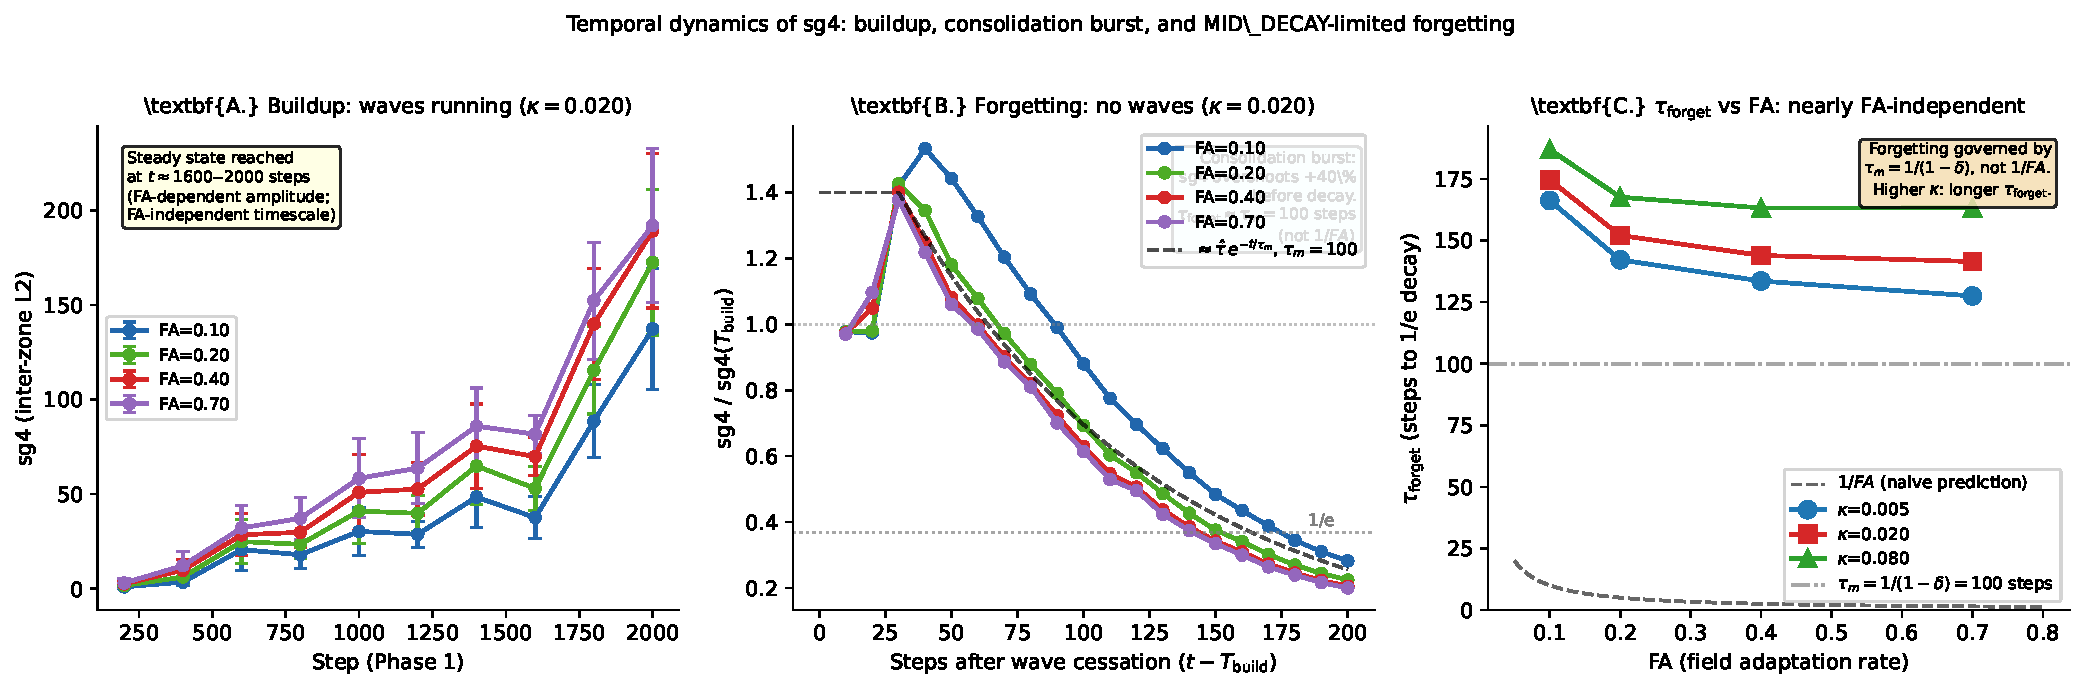
\includegraphics[width=\textwidth]{paper18_figure1.pdf}
\caption{\textbf{Temporal dynamics of VCML spatial structure.}
\textbf{A}: sg4 buildup during Phase~1 (waves running).
Steady state is approached around $t\approx1600$--$2000$ steps.
Higher FA reaches higher amplitude; timescales are similar.
\textbf{B}: sg4 normalized to value at wave cessation ($T_{\rm build}=2000$),
during Phase~3 (no waves, 5 seeds $\pm$ s.e.m., $\kappa=0.020$).
The consolidation burst ($\sim$40\% overshoot) is visible in the first 30 steps;
subsequent decay follows $\tau_m = 100$ steps (dashed).
\textbf{C}: Forgetting timescale $\tau_{\rm forget}$ vs FA for three $\kappa$ values.
Empirical points are nearly FA-independent (flat, $\sim$140--190 steps),
contradicting the naive prediction $1/\mathrm{FA}$ (black dashes, steep).
Higher $\kappa$ produces longer $\tau_{\rm forget}$.}
\label{fig:main}
\end{figure}

\end{document}
